
%(BEGIN_QUESTION)
% Copyright 2009, Tony R. Kuphaldt, released under the Creative Commons Attribution License (v 1.0)
% This means you may do almost anything with this work of mine, so long as you give me proper credit

Anta at vi bruker en reguleringsventil til å strupe strømningen av råolje gjennom en varmeovn fyrt med naturgassbrennere:

$$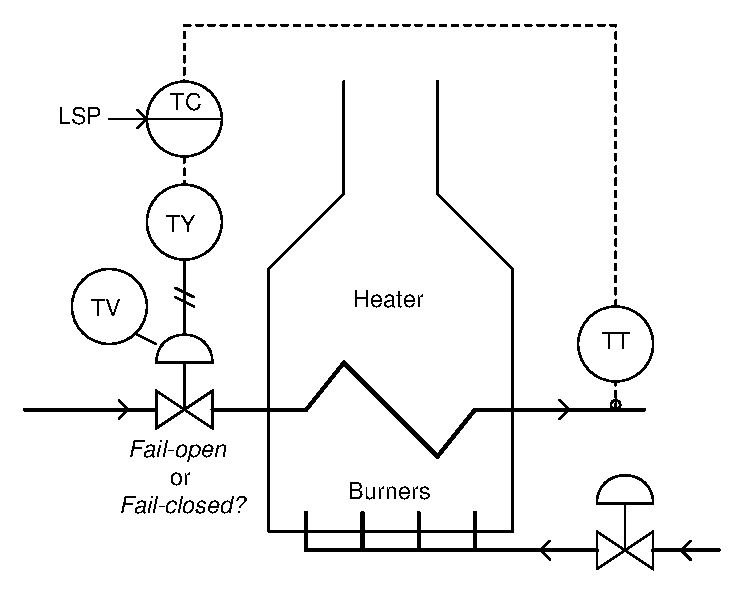
\includegraphics[width=15.5cm]{i00793x01.eps}$$

Strømningen reguleres normalt basert på råoljens utgående temperatur fra varmeovnen. I denne applikasjonen, bør vi velge en ventil som feiler lukket eller feiler åpen? Hvorfor? Og dersom ventilen drives av en pneumatisk fjær-membran-enhet, blir dette en luft-for-å-lukke- eller luft-for-å-åpne-ventil?

Til slutt, når du har bestemt riktig feilmodus for ventilen, bestem riktig reguleringsvirkning (direkte eller revers) for regulatoren.

\vskip 20pt \vbox{\hrule \hbox{\strut \vrule{} {\bf Forslag til sokratisk diskusjon} \vrule} \hrule}

\begin{itemize}
\item{} Beskriv en trinnvis strategi for å analysere slike systemer, slik at du {\it vet} at du har kommet frem til riktig svar.
\item{} For deg som har studert temperaturtransmittere med termoelement: avgjør om TT bør konfigureres for {\it upscale} eller {\it downscale} burnout.
\end{itemize}

\underbar{file i00793}
%(END_QUESTION)





%(BEGIN_ANSWER)

Vi bør velge en ventil som feiler åpen, noe som innebærer en luft-for-å-lukke-ventil (ved pneumatisk aktuering). Hvis ventilen i stedet feilet lukket, ville ovnsrørene kunne overopphetes og forårsake lekkasje av råolje over naturgassbrennerne, noe som kan gi stor brann. Når ventilen feiler fullt åpen, kjøles ovnsrørene ned og risikoen for rørbrudd reduseres.

Maksimal strømning gjennom ovnsrørene kan imidlertid også skape andre prosessproblemer, som flooding i destillasjonskolonnen. En alternativ løsning er å bruke en ventil som feiler lukket (luft-for-å-åpne), men med minimumsstrømningsstopp som hindrer ventilen i å lukke helt.

En annen alternativ løsning er å installere en manuell {\it bypass}-ventil parallelt med reguleringsventilen, og låse den manuelle ventilen i en lavstrømsstilling. På den måten vil det fortsatt gå en minimumsstrøm av råolje gjennom ovnsrørene når den feilsikre, feiler-lukket-reguleringsventilen går helt igjen. Hvis driftspersonell faktisk ønsker å stoppe strømningen helt, kan de låse opp den manuelle ventilen og stenge den også.

\vskip 10pt

Hvis transmitterledningene ryker, vil PV-signalet falle under null prosent. Da vil utgangen fra en reversvirkende regulator gå {\it opp}, og i dette tilfellet vil reguleringsventilen drives mot stengt stilling. Det er tydeligvis ikke feilmodusen vi ønsket når vi spesifiserte en luft-for-å-lukke-ventil.

Den beste løsningen er å konfigurere temperaturtransmitteren for revers virkning og regulatoren for direkte virkning. Med andre ord: stigende temperatur skal gi lavere 4-20 mA-signal. Da vil en åpen feil i transmitterkablene fremstå som høy temperatur ($>$ 100\%) for regulatoren, som med direkte virkning vil senke utgangen og la ventilen gå til sin hvilestilling (failsafe).

%(END_ANSWER)





%(BEGIN_NOTES)


%INDEX% Final Control Elements, valve: fail safe
%INDEX% Process: crude oil heater (fired)

%(END_NOTES)
